


The motivation for this stone is based on Burstedde et al (2008) \cite{bugg08}:

\begin{center}
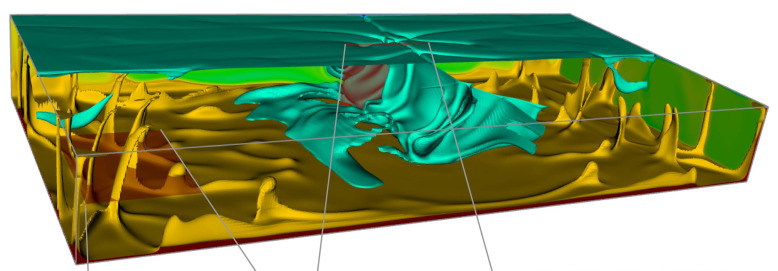
\includegraphics[width=12cm]{python_codes/fieldstone_88/images/bugg08}\\
{\captionfont Taken from \cite{bugg08}. Dimensionless dimensions are 8x4x1.}
\end{center}

This stone solves the dimensionless thermo-mechanical equations:
\begin{eqnarray}
\vec\nabla\cdot\vec\upnu &=& 0 \\
-\vec\nabla p + \vec\nabla \cdot [ 2 \eta(T,\dot{\varepsilon}_e,y) \dot{\bm \varepsilon} ] &=& Ra\; T \vec{e}_y \\
\frac{\partial T}{\partial t} + \vec\upnu \cdot \vec\nabla T &=& \Delta T
\end{eqnarray}
with $\dot{\varepsilon}_e$ is the effective strain rate and the viscosity $\eta$ is a simple
piecewise function of temperature, depth and strain rate.

This approach is not unique and we therefore look into two other similar implementations.

%------------------------------------------------------
\begin{center}
$----------------------------------$\\
$\smile \frown \bullet \circ \bullet \subset ( {\tt viscosity\_model=1} ) \supset \circ \bullet \smile \frown$\\
$----------------------------------$
\end{center}

The viscosity in Burstedde et al (2008) \cite{bugg08} is given by 
\[
\eta(T,\dot{\varepsilon}_e,y) =
\left\{
\begin{array}{c}
\min \left(  \frac{\sigma_y}{2 \dot{\varepsilon}_e} , 10\exp(-6.9T)  \right) \qquad y\le 0.9 \\
0.8 \exp(-6.9T) \qquad\quad  0.77\le y \le 0.9 \\
50 \exp(-6.9T) \qquad\quad y \le 0.77 
\end{array}
\right.
\]

\begin{center}
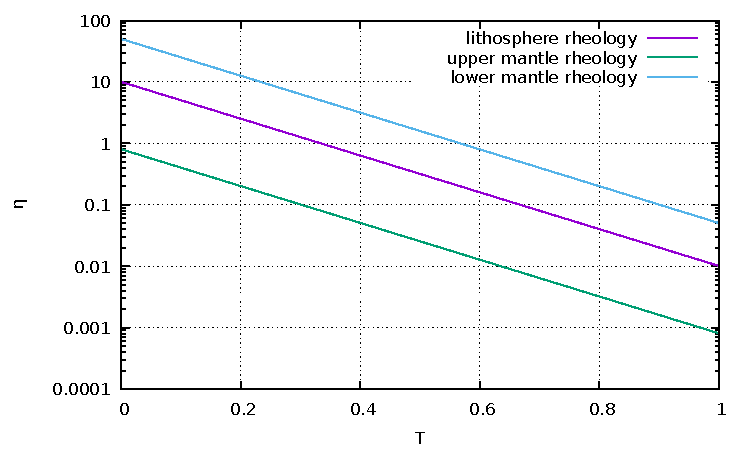
\includegraphics[width=8cm]{python_codes/fieldstone_88/images/visc.pdf}\\
{\captionfont Dimensionless viscosity values as a function of the dimensionless temperature.}
\end{center}

In the paper the value of $\sigma_y$ is not specified, nor is the Rayleigh number (although 
they mention it is between $10^6$ and $10^9$).
Their box is 8x4x1 and temperatures range from 0 at the top to 1 at the bottom.
In this case 3D modeling is out of the question here so we restrict ourselves to 2D with a 4x1 domain. 
We set $\sigma_y=1.5\cdot 10^5$ and $Ra=10^6$.

The initial temperature is based on the steady state conduction profile $T_(y)=1-y$, to which a
perturbation $\delta T(x,y)$ is added with 
\[
\delta T(x,y) = -0.03 \left[ \cos\left(2.132\pi \frac{x}{L_x}\right)
+ \cos\left(3.333\pi  \frac{x}{L_x}\right)
+ \cos\left(7.123 \pi  \frac{x}{L_x} \right) \right] \sin \left(\pi  \frac{y}{L_y} \right)
\]
The exact form of this perturbation is not critical, but it serves as a predictable and repeatable way of 
initiating the convection.

To start with, we implement the advection-diffusion equation without stabilisation but it is clear that 
large under- an overshoots occur due to the advection dominated heat transport in the large upwelling 
generated by the perturbation.

We then apply the Lenardic \& Kaula (1993) \cite{leka93} filter, as explained in Section~\ref{sec:compfield}.
\begin{enumerate}
\item Compute the initial sum $S_0$ of all values of $C$.
\item Find the minimal value $C_{min}$ below 0.
\item Find the maximal value $C_{max}$ above 1.
\item Set $C_i=0$ if $C_i \leq |C_{min}|$.
\item Set $C_i=1$ if $C_i \geq 2-C_{max}$. 
\item Compute the sum $S_1$ of all values of $C$
\item Compute the number $num$ of $0 < C_i < 1$.
\item Add $(S_1-S_0)/num$ to all $0<C_i<1$
\end{enumerate}

The filter is designed to prevent under- and overshoot but it cannot remove the oscillations between 0 and 1.
It therefore cannot 'cure' alone the poor quality of the solution within these bounds.
\begin{center}
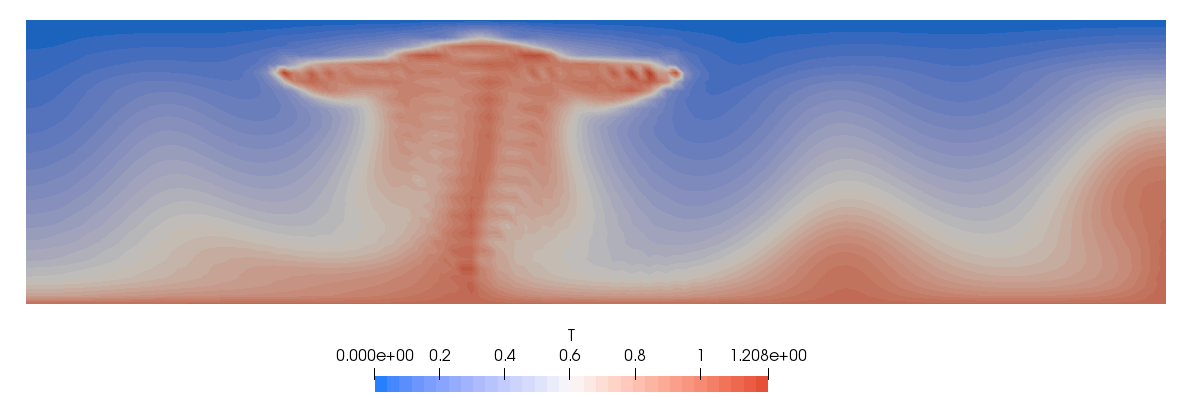
\includegraphics[width=9cm]{python_codes/fieldstone_88/results/without}\\
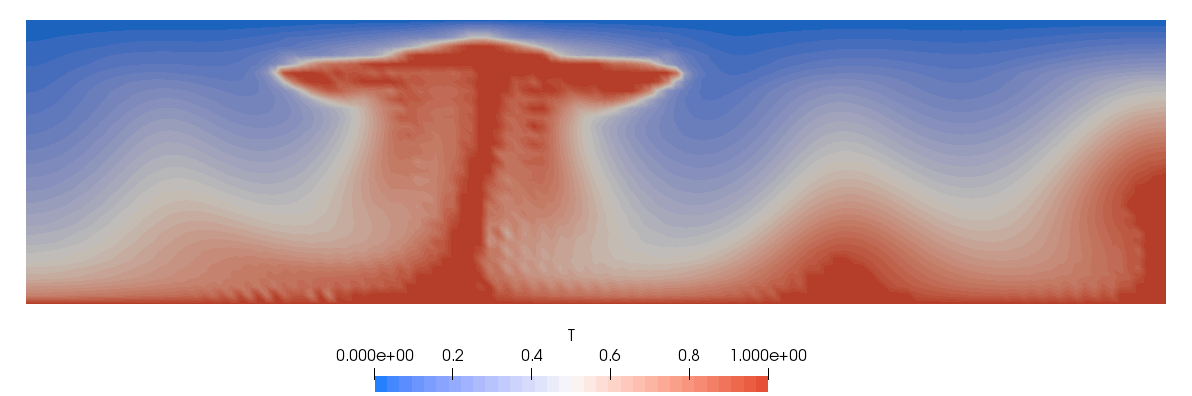
\includegraphics[width=9cm]{python_codes/fieldstone_88/results/with}\\
{\captionfont Top: no filter, bottom: with filter. 64x16, CFL=0.5\\ Notice the different scales.}
\end{center}

We now switch the filter off implement the SUPG method (see Section~\ref{ss:supg}). 
The resolution is set to 200x50:
\begin{center}
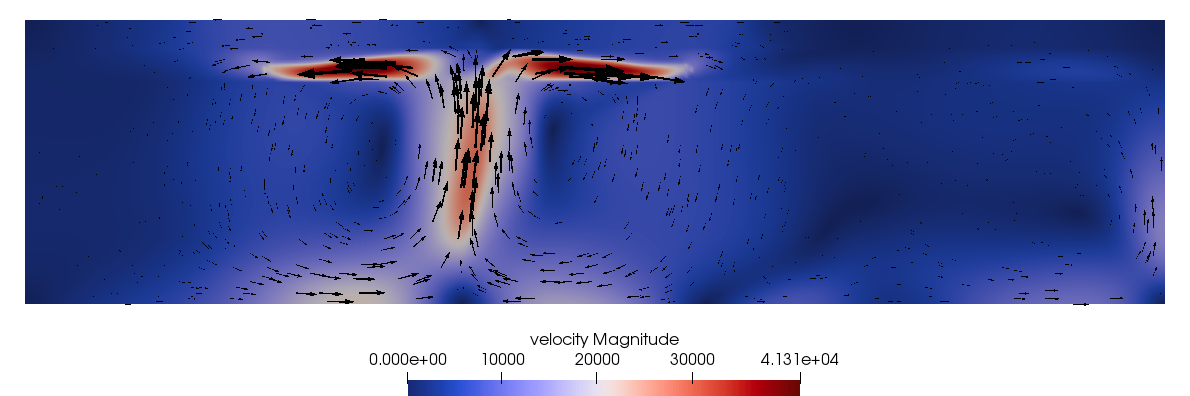
\includegraphics[width=8cm]{python_codes/fieldstone_88/results/200x50/vel}\\
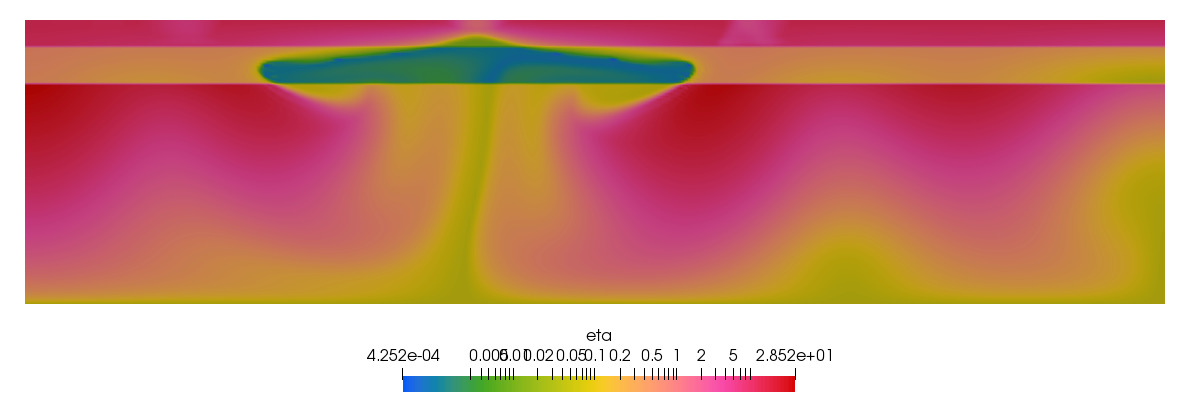
\includegraphics[width=8cm]{python_codes/fieldstone_88/results/200x50/eta}\\
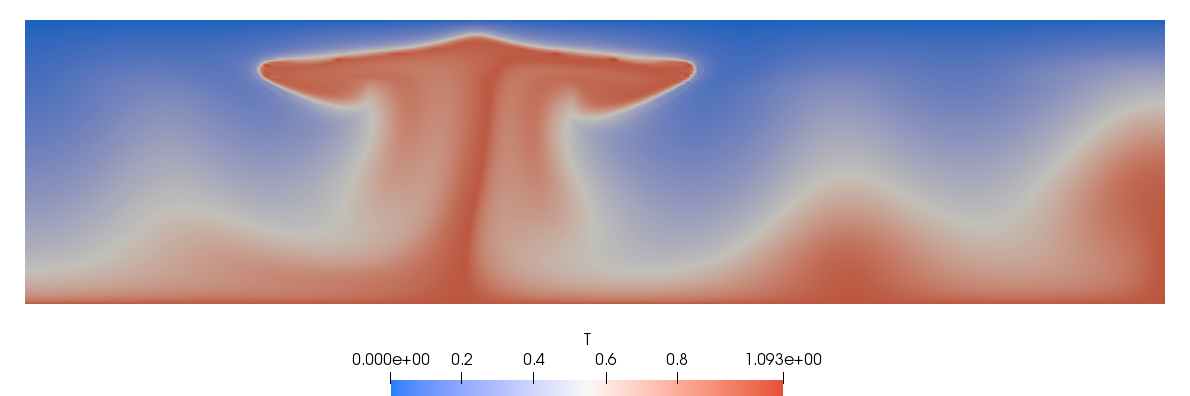
\includegraphics[width=8cm]{python_codes/fieldstone_88/results/200x50/T}\\
{\captionfont Velocity, viscosity and temperature fields at time $t\sim 0.00015$, CFL=0.5} 
\end{center}
We see that a combination of high-resolution and SUPG stabilisation keeps the 
temperature field within reasonable bounds. 


It is well known that in a well-mixed mantle, the average temperature profile 
follows the so-called adiabatic profile in its middle and that there are two 
boundary layers at the top and bottom. This adiabatic profile temperature gradient 
is much smaller than the conductive profile we start with.
We therefore revisit the topic of the initial temperature field and now start 
from a constant background temperature set to 0.5. 

The diffusion boundary layers are prescribed by means of a half-space cooling equation.
A rather artificial 'age' is set to $age=10^{-3}$ (the diffusion coefficient is 1, 
see dimensionless equations above).
The initial temperature is then obtained as follows: 1) set temperature everywhere to 0.5; 
2) add half-space cooling contribution to generate a field that smoothly transitions 
from 0.5 to 0 at the top and 0.5 to 1 at the bottom; 3) add perturbation. 

\begin{lstlisting}
for i in range(0,NV):
    T[i]=0.5
    T[i]-=0.5*special.erfc((Ly-yV[i])/2/np.sqrt(1*0.001))
    T[i]+=0.5*special.erfc(yV[i]/2/np.sqrt(1*0.001))
    T[i]-=0.03*(np.cos(2.132*np.pi*xV[i]/Lx)+\
                np.cos(3.333*np.pi*xV[i]/Lx)+\
                np.cos(7.123*np.pi*xV[i]/Lx)) *np.sin(np.pi*yV[i]/Ly)
\end{lstlisting}


In what follows we set CFL=0.5 and SUPG is used.
We see that the behaviour of the system is very different. The perturbation generates 
much smaller buoyancy forces. The huge upwelling is gone and rather plumes form. 

INCLUDE PICS


Also, in order to better visusalise the flow, we add passive markers which are 
advected with the computed velocity at each time step (see fieldstone 37).
These are painted with a checkerboard pattern.



%------------------------------------------------------
\begin{center}
$----------------------------------$\\
$\smile \frown \bullet \circ \bullet \subset ( {\tt viscosity\_model=2} ) \supset \circ \bullet \smile \frown$\\
$----------------------------------$
\end{center}

We can also explore a different rheology, as given in Brandenburg et al (2008) \cite{brhv08}:
\[
\eta(y,T) = \eta_0(y) \exp [-b(cT)]
\]
with 
\[
\left\{
\begin{array}{c}
\eta_0(y)=1000, c=0 \qquad y> 0.9551 \\
\eta_0(y)=1,    c=1, \qquad  0.7187  <y< 0.9551 \\
\eta_0(y)=30,   c=1  \qquad\quad y \le 0.0.7187
\end{array}
\right.
\]
and $b=\ln 1000$.

%------------------------------------------------------
\begin{center}
$----------------------------------$\\
$\smile \frown \bullet \circ \bullet \subset ( {\tt viscosity\_model=3} ) \supset \circ \bullet \smile \frown$\\
$----------------------------------$
\end{center}


A similar yet different rheology is found in Zhang et al (2010) \cite{zhzl10}:
\[
\eta(y,T) = \eta_0(y) \exp [A(0.5-T)]
\]
with $A=9.2103$. The expression for $\eta_0(r)$ is given in the text (section 3.1):
"The depth‐dependent prefactors $\eta_0(r)$ in equation (9)
for the lithosphere and the upper mantle are 1 and 1/30,
respectively. For the lower mantle, $\eta_0(r)$ increases
linearly from 2.0 at the 670 km depth to 6.8 at the CMB. This
leads to a mantle viscosity structure in which the lower mantle
viscosity on average is $\sim 2$ orders of magnitude higher than
that in the upper mantle." Note that is corresponds to case FS1 in the paper. 

The base of the lithosphere is set to 120km, so its dimensionless
vertical coordinate is 
\[
y_l = \frac{2891-120}{2891} \simeq 0.9585
\] 
The base of the upper mantle is set to 670km, so its dimensionless
vertical coordinate is 
\[
y_{um} = \frac{2891-670}{2891} \simeq 0.7682
\] 
Finally the expression for $\eta_0(r)$ in the lower mantle 
is 
\[
\eta_0(y)= - \frac{6.8-2}{y_{um}} y + 6.8 = -6.24837 y + 6.8
\]

\begin{center}
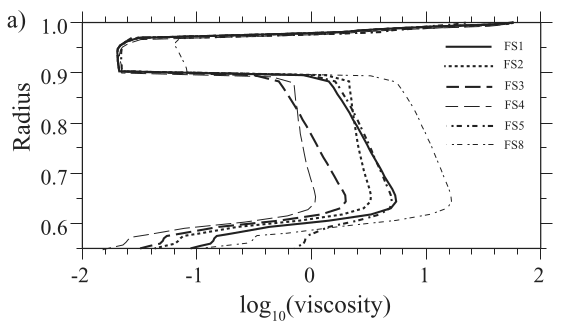
\includegraphics[width=7cm]{python_codes/fieldstone_88/images/zhzl10a}
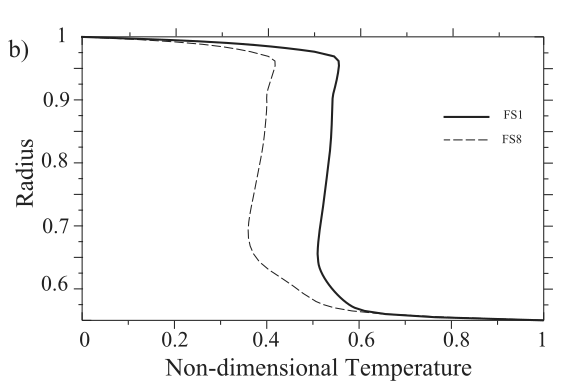
\includegraphics[width=7cm]{python_codes/fieldstone_88/images/zhzl10b}\\
{\captionfont Taken from Zhang et al (2010) \cite{zhzl10}.
Depth dependences of horizontally averaged
(a) mantle viscosities for cases FS1, FS2, FS3, FS4, FS5,
and FS8 and (b) mantle temperatures for cases FS1 and FS8.}
\end{center}


 



\vspace{2cm}

\note{
Problems \& ToDos: \\
pressure nullspace \\
nonlinear iterations missing\\
As usual code is painfully slow...
}
